
% --------------------------------------------------------------------------------------
%                   LATEX TEMPLATE FOR DISSERTATION (HONS)
% --------------------------------------------------------------------------------------
\documentclass[11pt]{book}

\usepackage{amsfonts, amsmath, amssymb}  
\usepackage{times}

%\usepackage[backref=page,pagebackref=true,linkcolor = blue,citecolor = red]{hyperref}
%\usepackage[backref=page]{backref}


\usepackage{graphicx}
\DeclareGraphicsExtensions{.pdf,.png,.jpg}


\setlength{\oddsidemargin}{1.5cm}
\setlength{\evensidemargin}{0cm}
\setlength{\topmargin}{1mm}
\setlength{\headheight}{1.36cm}
\setlength{\headsep}{1.00cm}
%\setlength{\textheight}{20.84cm}
\setlength{\textheight}{19cm}
\setlength{\textwidth}{14.5cm}
\setlength{\marginparsep}{1mm}
\setlength{\marginparwidth}{3cm}
\setlength{\footskip}{2.36cm}


\begin{document}
\pagestyle{empty}

%: ----------------------------------------------------------------------
%:                  TITLE PAGE: name, degree,..
% ----------------------------------------------------------------------


\begin{center}

\vspace{1cm}

%%% Type the thesis title below%%%%%%%%%%%%%%%%
{\Huge         Nested sampling with peers}

\vspace{35mm} 


\includegraphics[width=2cm]{logo}

 \vspace{45mm}

%%%%%Type Your Name Below%%%%%%%%%%%%
{\Large       Feishuang Wang}

	\vspace{1ex}

School of Computer Science

The University of Auckland

	\vspace{5ex}

 %%%%%Typing Your Supervisors Name Below%%%%%%%%%%%%
Supervisor:             Dr Brendon James Brewer

	\vspace{30mm}

A dissertation  submitted in partial fulfillment of the requirements for the degree of Master of Professional Studies in Data Science OR Master of Data Science (delete one), The University of Auckland, 20XX.

\end{center}


  \newpage



%: --------------------------------------------------------------
%:                  FRONT MATTER:  abstract,..
% --------------------------------------------------------------
\chapter*{Abstract}       
\setcounter{page}{1}
\pagestyle{headings}
% \pagenumbering{roman}

\addcontentsline{toc}{chapter}{Abstract}
A nested sampling algorithm is a Bayesian approach to computing and comparing models and generating samples from posterior distributions. We introduce a general Monte Carlo method based on Nested Sampling, which name is Nested Sampling with peers, this method generates one particle above the threshold from the last iteration by querying the params from the server and updating it. We describe the new method over a test case and find that it has better accuracy than the original MCMC-based nested sampling with the same computational overhead.
 Put your abstract  here.  
 The abstract should contain a brief summary of the aim, methodologies, 
finding and conclusions of the dissertation.  The abstract should normally be fewer than 350 words.



%: --------------------------------------------------------------
%:                  END:  abstract
% --------------------------------------------------------------


%: ----------------------- contents ------------------------
\setcounter{secnumdepth}{3} % organisational level that receives a numbers
\setcounter{tocdepth}{3}    % print table of contents for level 3
\tableofcontents            % print the table of contents
% levels are: 0 - chapter, 1 - section, 2 - subsection, 3 - subsection



%: --------------------------------------------------------------
%:                  MAIN DOCUMENT SECTION
% --------------------------------------------------------------
	
\chapter{Introduction}%    \chapter{}  = level 1, top level

\section{Bayesian Analysis} 
The Bayesian Analysis problem is in fact a parameter estimation problem, 
The term \textit{parameter} means \textit{unknown quantity}, howerver in real world, we don't 
have enough information to decide a quantity, so we need Bayesian Analysis to help us.
The parameter you interested in are denoted by $\theta$, to estimate them, first of all, you need to 
model a probability distribution on the \textit{hypothesis space}, a \textit{hypothesis space} is the 
collection of possibilities, this means that you are modeling the initial assumptions, and the probability distribution
is called the \textit{prior}, it is the distribution of $\theta$. The data set is called D, 
after that we can use Bayes’ Theorem to determine the \textit{posterior distribution}:
\begin{equation}
	p(\theta|D) = \frac{p{(\theta)}p(D|\theta)}{p(D)}
\end{equation}
in the above equation, 
\begin{enumerate}
	\item $p(\theta|D)$ is the posterior distribution, the conditional distribution of $\theta$ given the observed data, $D$.
 \item $p{(\theta)}$ is prior distribution specified based on prior assumptions or information
 \item $p(D|\theta)$ is the likelihood which refers to the conditional
 probability of observing the data
 \item  $p(D)$ is the marginal likelihood (or evidence) that refers to the probability of $D$
 regardless of the values of $\theta$.
\end{enumerate}


\subsection{Marginal Likelihood}
% The main strength of LaTex is  mathematical typesetting.  

% There is a huge amount of information about LaTex on the internet.
% A helpful short manual, also included in this folder, is the file
% \verb+latex_intro.pdf+
% This document gives a lot of sample LaTex commands.  
% The file \verb+latex-howto.tex+ in this folder also contains examples of many latex commands.
\section{Nested Sampling} 
\section{Distributed System}
\subsection{BONIC}
\section{Spakslab Problem}

\chapter{Implementation}
We first show  some simple examples of 
mathematical formulae using latex typesetting.

\begin{enumerate}
\item The basic functions: $\cos(x),  \sin(x),   \ln(x) $,  (\verb+$\cos(x),\sin(x),\ln(x)$+). 
\item Greek letters: $\alpha \beta \gamma \delta\epsilon...$ (\verb+$\alpha\beta\gamma\delta\epsilon...$+).
\item Mathematical symbols: $\int  \oint \sum\lim\bigcup \bigcap$
 (\verb+$\int\oint\sum\lim\bigcup\bigcap$+).
\item Fractions: $\frac{1}{2},\frac{1}{2-x}$ (\verb+$\frac{1}{2},\frac{1}{2-x}$+).
\end{enumerate}

The following matrix 
\begin{eqnarray}\label{eqn:matrix}
\left[
\begin{array}{ccc}
	 U_{r}&     r       &   W_{r}	\\
	   0       &	1      &  V_{x}	\\
	   0	   &	0      &  W_{x}
\end{array}
\right], 
\end{eqnarray}
is generated using  the \verb+equarray+ environment:
\begin{verbatim}
\begin{eqnarray}\label{eqn:matrix}
\left[
\begin{array}{ccc}
	 U_{r}& r &W_{r}\\
	   0 &1 &V_{x}\\
	   0&	0 & W_{x}
\end{array}
\right], 
\end{eqnarray}
\end{verbatim}
The \verb+\label{eqn:matrix}+ command labels the equation with \verb+{eqn:matrix}+ which can 
be referred  to somewhere else in the text by using \verb+\ref{eqn:matrix}+ or  \verb+\eqref{eqn:matrix}+.


The command \verb+\notag+ eliminates the numbering of the first equation,
\begin{eqnarray} \label{eqn:lambda_trace}
\lambda^{(1)}&=&tr[T^{(1)}P],\notag  \\
\lambda^{(2)}&=&tr[T^{(2)}P - T^{(1)}ST^{(1)}P].
\end{eqnarray}
\begin{verbatim}
\begin{eqnarray} \label{eqn:lambda_trace}
\lambda^{(1)}&=&tr[T^{(1)}P],\notag  \\
\lambda^{(2)}&=&tr[T^{(2)}P - T^{(1)}ST^{(1)}P].
\end{eqnarray}
\end{verbatim}


\subsection{Itemized lists}
Example of an itemized list:
\begin{itemize}
\item muscle and fat cells remove glucose from the blood,
\item cells use glucose for protein synthesis.
\end{itemize}
\begin{verbatim}
\begin{itemize}
\item muscle and fat cells remove glucose from the blood,
\item cells use glucose for protein synthesis.
\end{itemize}
\end{verbatim}
This can be done by an enumerated  list:
\begin{enumerate}
\item muscle and fat cells remove glucose from the blood,
\item cells use glucose for protein synthesis.
\end{enumerate}

\begin{verbatim}
\begin{enumerate}
\item muscle and fat cells remove glucose from the blood,
\item cells use glucose for protein synthesis.
\end{enumerate}
\end{verbatim}



\newpage



\subsection{Inserting figures}


You may save your Matlab figures as jpg files.  Figures should  be stored in the 
same folder as the latex files.
For the graphicx package to work you usually need to ask latex to create a pdf file (e.g., command pdflatex or latexpdf).

An example of an inserted image is given in Figure~\ref{fig:modes}.

\begin{center}
\begin{figure}[h]
		\centering
		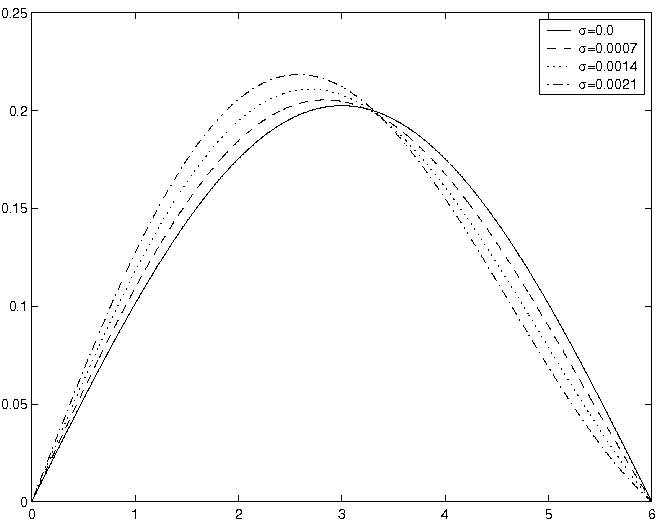
\includegraphics[width=0.6\textwidth]{modes}
		\caption{Mode shapes}
		\label{fig:modes}
\end{figure}
\end{center}




 
\subsection{Tables}\label{table}
Example of a table,
\begin{table}[htp]
\centering
\begin{tabular}{ccc} % ccc means 3 columns, all centered; alternatives are l, r
{\bf Gene} & {\bf GeneID} & {\bf Length} \\ 
\hline % draws a line under the column headers
human latexin & 1234 & 14.9 kbps \\
mouse latexin & 2345 & 10.1 kbps \\
rat latexin   & 3456 & 9.6 kbps \\
\end{tabular}
\caption[title of table]{\textbf{title of table} - Overview of latexin genes.}
\label{latexin_genes} % label for cross-links with \ref{latexin_genes}
\end{table}
\begin{verbatim}
\begin{table}[htp]
\centering
\begin{tabular}{ccc} 
% ccc means 3 columns, all centered; alternatives are l, r
{\bf Gene} & {\bf GeneID} & {\bf Length} \\ 
\hline % draws a line under the column headers
human latexin & 1234 & 14.9 kbps \\
mouse latexin & 2345 & 10.1 kbps \\
rat latexin   & 3456 & 9.6 kbps \\
\end{tabular}
\caption[title of table]{\textbf{title of table} - Overview of latexin genes.}
\label{latexin_genes} % label for cross-links with \ref{latexin_genes}
\end{table}
\end{verbatim}
See how to add two vertical lines in the table (Simply change \verb+{ccc}+ to \verb+{c|c|c}+)
\begin{table}[htp]
\centering
\begin{tabular}{c|c|c} % ccc means 3 columns, all centered; alternatives are l, r
{\bf Gene} & {\bf GeneID} & {\bf Length} \\ 
\hline % draws a line under the column headers
human latexin & 1234 & 14.9 kbps \\
mouse latexin & 2345 & 10.1 kbps \\
rat latexin   & 3456 & 9.6 kbps \\
\end{tabular}
\caption[title of table]{\textbf{title of table} - Overview of latexin genes.}
\label{latexin_genes2} % label for cross-links with \ref{latexin_genes}
\end{table}





\subsection{How to Refer to Equations, Sections, etc}%    \subsection{}    = level 3
 \begin{enumerate}
 \item References can be linked to equations, figures, tables or sections using the command 
 \verb+\ref+:
 Equation (\ref{eqn:lambda_trace}),  Figure~\ref{fig:modes},  Table~\ref{latexin_genes2} and Section~\ref{table}.\\
\verb+Equation~(\ref{eqn:lambda_trace}),Figure~\ref{modes},+\\
\verb+Table~\ref{latexin_genes2} and Section~\ref{table}.+


\item 
Equations can be conveniently  referred to using \verb+ \eqref+. See, for example,  Equation \eqref{eqn:lambda_trace}. \\
\verb+Equation \eqref{eqn:lambda_trace}+\\
Note that \verb+\eqref+ includes the round brackets by itself. 

\item  Citations are in a similar way but using the command \verb+\cite+:

  \cite{Salmond}, \cite{Stull}, and \cite{TandC}, 
   or  \cite{Salmond,Stull,TandC} .
   
  \begin{verbatim}   
   \cite{Salmond}, \cite{Stull}, and \cite{TandC}, 
   or  \cite{Salmond,Stull,TandC} .
 \end{verbatim} 

There are many different styles for writing citations -- you should follow the norms for your subject area.

A more advanced way to do citations is to use \verb+bibtex+.  This is a powerful tool and we encourage you to try it.  There is plenty of information about it on the web.

 
 \end{enumerate}
 
 
 
\chapter{Methodologies and analysis}
\section{Methodologies}
\section{Analysis}
\chapter{Discussion }
\section{Main results}
\section{Discussion}
\chapter{Conclusions}
You may add more chapters as needed in the file.

% --------------------------------------------------------------

% --------------------------------------------------------------
\renewcommand{\bibname}{References} % changes the header; default: Bibliography
\begin{thebibliography}{99} 
\addcontentsline{toc}{chapter}{References}


\bibitem{Farge} Farge Marie, {\em Wavelet Transforms and Their Applications to Turbulence},  \\Ann. Rev. Fluid Mech. volume 24, pages 395-457, 1992.
%ref. for an article
\bibitem{Salmond}  Salmond Jennifer,  {\em Vertical Mixing of Ozone in the Very Stable Nocturnal Boundary Layer}, PhD Thesis, University of British Columbia, 2001.
%ref. for a Thesis.
\bibitem{Stull} Stull B. Ronald, {\em Introduction to Boundary Layer Meteorology}, Dordrecht; Boston: Kulwer Academic Publishers, 1988. %%%ref. for a book
\bibitem{TandC} Torrence Christopher, Compo Gilbert P., {\em A Practical Guide to Wavelet Analysis}, Bulletin of the American Meteorological Society volume 79, pages 61-78, 1998. 
%ref. for an article
\end{thebibliography}


\appendix%%% start appendices here 
\chapter{Some extra things} 

This is an optional chapter for any additional material that does not fit 
conveniently into the body of the text (e.g., data, copies of computer programmes). 
Note that appendices won't necessarily be marked.


\end{document}
